% Copyright (C) 2017 Mario Sanchez Prada
% Author: Mario Sanchez Prada <mario@mariospr.org>
%
% This presentation is distributed under the terms of the 
% Creative Commons Attribution-ShareAlike 2.0:
%
%     http://creativecommons.org/licenses/by-sa/2.0/
%

\section{Flatpak}
\subsection{What is Flatpak?}

\begin{frame}
  \frametitle{\insertsubsection}

    \begin{itemize}
    \item A new way of distributing applications in Linux\vspacing
    \item Sits on top of OSTree and \textit{bubblewrap} (chroot on steroids)\vspacing
    \item Allows having both user and system-wide installations\vspacing
    \item Cross-platform by design: \textbf{runtimes} and \textbf{applications}\vspacing
    \item Reliable and secure: GPG signatures, sanboxing, portals...\vspacing
    \item Open Source project. Started by Red Hat, contributions from Endless, Collabora, Codethink, Intel, Kinvolk, Solus...
    \end{itemize}

    \begin{flushleft}
      Similar in some ways to Docker, but with the focus on end user
      applications instead of for containerized system-wide services.
    \end{flushleft}
\end{frame}

\subsection{A brief note on bubblewrap}

\begin{frame}[fragile]
  \frametitle{\insertsubsection}

    \begin{itemize}
    \item Allows running sandboxed applications in chroot-like environments as an \textbf{unprivileged user}\vspacing
    \item Creates a mount namespace with \texttt{/} on a \texttt{tmpfs}\vspacing
    \item Uses \texttt{PR\_SET\_NO\_NEW\_PRIVS} when cloning the process to limit what the binary can do after dropping privileges\vspacing
    \item Implements a subset of the Kernel's user namespaces feature to isolate processes\vspacing
    \item More namespaces: \small{\texttt{CLONE\_NEWUSER}, \texttt{CLONE\_NEWIPC}, \texttt{CLONE\_NEWPID}, \texttt{CLONE\_NEWNET}, \texttt{CLONE\_NEWUTS}}\vspacing
    \item Allows passing a list of \textit{seccomp} filters to limit \textit{syscalls}\vspacing
    \end{itemize}

\end{frame}

\subsection{Bubblewrap example}

\begin{frame}[fragile]
  \frametitle{\insertsubsection}
\begin{tiny}
\begin{verbatim}
[fedoravm ~]$ bwrap --ro-bind /usr /usr --ro-bind /etc/resolv.conf /etc/resolv.conf \
       --symlink usr/lib /lib --symlink usr/lib64 /lib64 --symlink usr/bin /bin \
       --dir /tmp --proc /proc --dev /dev \
       --unshare-pid --unshare-net \
       --chdir / \
       /bin/sh

sh-4.3$ ls /
bin  dev  etc  lib  lib64  proc  tmp  usr

sh-4.3$ ls /dev/
console  full  null  ptmx  pts	random	shm  stderr  stdin  stdout  tty  urandom  zero

sh-4.3$ ls -l /etc/
total 4
-rw-r--r-- 1 65534 65534 53 Mar 14 00:46 resolv.conf

sh-4.3$ ifconfig
lo: flags=73<UP,LOOPBACK,RUNNING>  mtu 65536
        inet 127.0.0.1  netmask 255.0.0.0
        inet6 ::1  prefixlen 128  scopeid 0x10<host>
        loop  txqueuelen 1  (Local Loopback)
        RX packets 0  bytes 0 (0.0 B)
        RX errors 0  dropped 0  overruns 0  frame 0
        TX packets 0  bytes 0 (0.0 B)
        TX errors 0  dropped 0 overruns 0  carrier 0  collisions 0

sh-4.3$ ps aux
USER       PID %CPU %MEM    VSZ   RSS TTY      STAT START   TIME COMMAND
1000         1  0.0  0.0  15472   160 ?        S    01:28   0:00 bwrap --ro-bind /usr /usr --ro-bind /etc/resolv.conf /etc/resolv.conf --symlink usr/lib /lib --symlink usr/lib64 /lib64 --symlink usr/bin /bin --dir /tmp --proc /proc --dev 
1000         2  0.0  0.1 122136  3608 ?        S    01:28   0:00 /bin/sh
1000         8  0.0  0.1 150020  3544 ?        R+   01:29   0:00 ps aux
\end{verbatim}
\end{tiny}
\end{frame}

\subsection{Anatomy of a Flatpak Runtime}
\begin{frame}[fragile]
  \frametitle{\insertsubsection}

    \begin{tiny}
\begin{verbatim}
           $ tree -L 3 /var/lib/flatpak/runtime/org.gnome.Platform/x86_64/3.22/active/
           |-- deploy
           |-- files
           | |-- bin
           | | |-- [...]
           | | |-- basename
           | | |-- bash
           | | |-- [...]
           | |-- etc
           | | |-- [...]
           | | |-- ca-certificates.conf
           | | |-- dbus-1
           | | |-- [...]
           | |-- lib
           | | |-- [...]
           | | |-- libglib-2.0.so.0.5000.2
           | | |-- libGL.so -> libGL.so.1.0.0
           | | |-- [...]
           | |-- lib64
           | | `-- ld-linux-x86-64.so.2 -> /usr/lib/ld-linux-x86-64.so.2
           | |-- [...]
           | |-- manifest-base-1.json
           | |-- manifest.json
           | |-- sbin -> bin
           | |-- share
           | | |-- [...]
           | | |-- applications
           | | |-- [...]
           | `-- var
           |     |-- cache
           |     |-- lib
           |     `-- run
           `-- metadata
\end{verbatim}
    \end{tiny}
\end{frame}

\subsection{Anatomy of a Flatpak Application}
\begin{frame}[fragile]
  \frametitle{\insertsubsection}

    \begin{tiny}
\begin{verbatim}
           $ tree -L 3 /var/lib/flatpak/app/org.gnome.Todo/current/active/
           /var/lib/flatpak/app/org.gnome.Todo/current/active/
           |-- deploy
           |-- export
           |   `-- share
           |       |-- applications
           |       |-- dbus-1
           |       `-- icons
           |-- files
           |   |-- bin
           |   |   `-- gnome-todo
           |   |-- lib
           |   |   |-- debug
           |   |   |-- evolution-data-server
           |   |   |-- girepository-1.0
           |   |   |-- gnome-todo
           |   |   |-- goa-1.0
           |   |   |-- libcamel-1.2.so -> libcamel-1.2.so.59.0.0
           |   |   |-- [...]
           |   |   `-- systemd
           |   |-- manifest.json
           |   `-- share
           |       |-- appdata
           |       |-- applications
           |       |-- dbus-1
           |       |-- GConf
           |       |-- gir-1.0
           |       |-- glib-2.0
           |       |-- icons
           |       |-- locale
           |       |-- pixmaps
           |       `-- runtime
           `-- metadata
\end{verbatim}
    \end{tiny}
\end{frame}

\subsection{Putting all together: running a flatpak app}
\begin{frame}[fragile]
  \frametitle{\insertsubsection}

    \begin{tiny}
\begin{verbatim}
  /.flatpak-info                                 [...]
  /app                                           /run/user/1000
      /app/bin                                   /run/user/1000/Xauthority
      /app/lib                                   /run/user/1000/app
      /app/share                                 /run/user/1000/app/org.gnome.Todo
      [...]                                      /run/user/1000/bus
  /bin                                           /run/user/1000/dconf
  /dev                                           /run/user/1000/dconf/user
      /dev/console                               /run/user/1000/doc
      /dev/full                                  /run/user/1000/flatpak-info
      /dev/null                                  [...]
      [...]                                  /sbin
  /etc                                      /sys
  [...]                                          /sys/block
  /home/mario                                    [...]
      /home/mario/.config                    /tmp
      /home/mario/.local/share/flatpak           /tmp/.X11-unix
      /home/mario/.var/app/org.gnome.Todo        /tmp/.X11-unix/X99
  /lib                                           [...]
  /lib64                                     /usr
  /local                                         /usr/bin
  /proc                                          /usr/share
      /proc/1                                    /usr/share/applications
      /proc/1/attr                               [...]
      [...]                                  /var
  /run                                           /var/cache
      /run/build                                 /var/config
      /run/build-runtime                         /var/config/user-dirs.dirs
      /run/host                                  [...]
      /run/systemd                               /var/data
      /run/user/1000                             /var/run
      [...]                                      /var/tmp
\end{verbatim}
    \end{tiny}
\end{frame}

\subsection{Platform and SDK Runtimes}
\begin{frame}
  \frametitle{\insertsubsection}

  Currently \textbf{two main standard runtimes} available:
  \begin{itemize}
  \item Freedesktop runtime: containes a set of essential libraries and services: D-Bus, GLib, PulseAudio, X11, Wayland\vspacing
  \item GNOME runtime: based on the Freedesktop runtime, adds libraries like GTK+, GStreamer or GVFS on top.
  \end{itemize}

  \begin{center}
    A KDE runtime is currently under development too:\\
    \small{\url{https://github.com/KDE/flatpak-kde-runtime}}\\\vspacing
  \end{center}

  Two \textbf{types of runtimes}:
  \begin{itemize}
    \item Platform runtime: just the bits needed to \textbf{run} apps\vspacing
    \item SDK runtime: platform + the necessary tools and files for development purposes (e.g. headers, debug symbols...)\vspacing
    \end{itemize}
\end{frame}

\subsection{The Sandbox}
\begin{frame}
  \frametitle{\insertsubsection}

  Limited access to the host system by default:
    \begin{itemize}
    \item No access to processes outside the sandbox (\textit{namespaces})\vspacing
    \item No access to the network, session bus and devices\vspacing
    \item Controlled execution of certain \textit{syscalls} (\textit{seccomp} filters)\vspacing
    \item Read-only access to the runtime and app (\textit{bind mounts})\vspacing
    \item Read-write access to \texttt{\$HOME/.var/app/\$APPID}\vspacing
    \item Controlled access to resources (\textit{cgroups})\vspacing
    \item No access to host services (e.g. X/Wayland, system bus...)
    \end{itemize}

    \begin{flushleft}
      Flatpak's sandbox is very limiting by default, but there are ways of dealing with that to run real-word applications...
    \end{flushleft}
\end{frame}

\subsection{Escaping the Sandbox: fine-grained permissions}
\begin{frame}[fragile]
  \frametitle{\insertsubsection}

  Easiest way to work with the sandbox is to open ``holes'' in it:
    \begin{itemize}
    \item Grant access to UNIX domain sockets: X.org, Wayland, PulseAudio, System and Sesssion D-Bus...\vspacing
    \item Grant access to specific devices: dri, kvm\vspacing
    \item Grant access to see, use and/or own specific D-Bus names\vspacing
    \item Share specific subsystems with the host (network, IPC)\vspacing
    \item Fine-grained permissions for filesystem access\vspacing
    \item Define extensions for runtimes or applications (e.g. l10n)
    \end{itemize}

    \begin{flushleft}
      Combining all this enables makes it possible to run apps in a more controlled way, but it's not very secure.
    \end{flushleft}
\end{frame}

\subsection{The manifest file}
\begin{frame}[fragile]
  \frametitle{\insertsubsection}

  A Flatpak manifest file (\texttt{metadata}):
    \begin{tiny}
\begin{verbatim}
           [Application]
           name=org.gnome.Calculator
           runtime=org.gnome.Platform/x86_64/3.20
           sdk=org.gnome.Sdk/x86_64/3.20
           command=gnome-calculator

           [Context]
           shared=network;ipc;
           sockets=x11;wayland;
           filesystems=xdg-run/dconf;~/.config/dconf:ro;

           [Session Bus Policy]
           ca.desrt.dconf=talk

           [Environment]
           DCONF_USER_CONFIG_DIR=.config/dconf

           [Extension org.gnome.Calculator.Locale]
           directory=share/runtime/locale
           subdirectories=true

           [Extension org.gnome.Calculator.Debug]
           directory=lib/debug
\end{verbatim}
    \end{tiny}
\end{frame}

\subsection{Escaping the sandbox: Portals}
\begin{frame}
  \frametitle{\insertsubsection}

  \begin{itemize}
  \item High-level APIs to allow sandboxed apps request access\vspacing
  \item Out-of-process services, run in the host system\vspacing
  \item Sandboxed apps communicate via D-Bus\vspacing
  \item Different types of portals for different needs:
    \begin{itemize}
    \item NetworkMonitor, OpenURI, Filechooser, Documents, Printing, Geolocation, Screenshots, Notifications, Proxy...\vspacing
    \end{itemize}

  \item Using portals is \textbf{safe}:
    \begin{itemize}
    \item They don't expose sensible information from the host\vspacing
    \item Portal-initiated operations are \textbf{interactive} an \textbf{cancellable}\vspacing
    \end{itemize}

  \item Split in UI-less frontend + desktop-specific backends:
    \begin{itemize}
    \item Currently backends for GTK+, with KDE work-in-progress.\vspacing
    \item GLib \& GTK+ include support for several portals since 3.22
    \end{itemize}
  \end{itemize}

\end{frame}

\subsection{An example of Portals}
\begin{frame}[fragile]
  \frametitle{\insertsubsection}

  \texttt{\$ flatpak run org.gnome.PortalTest}
  \begin{center}
    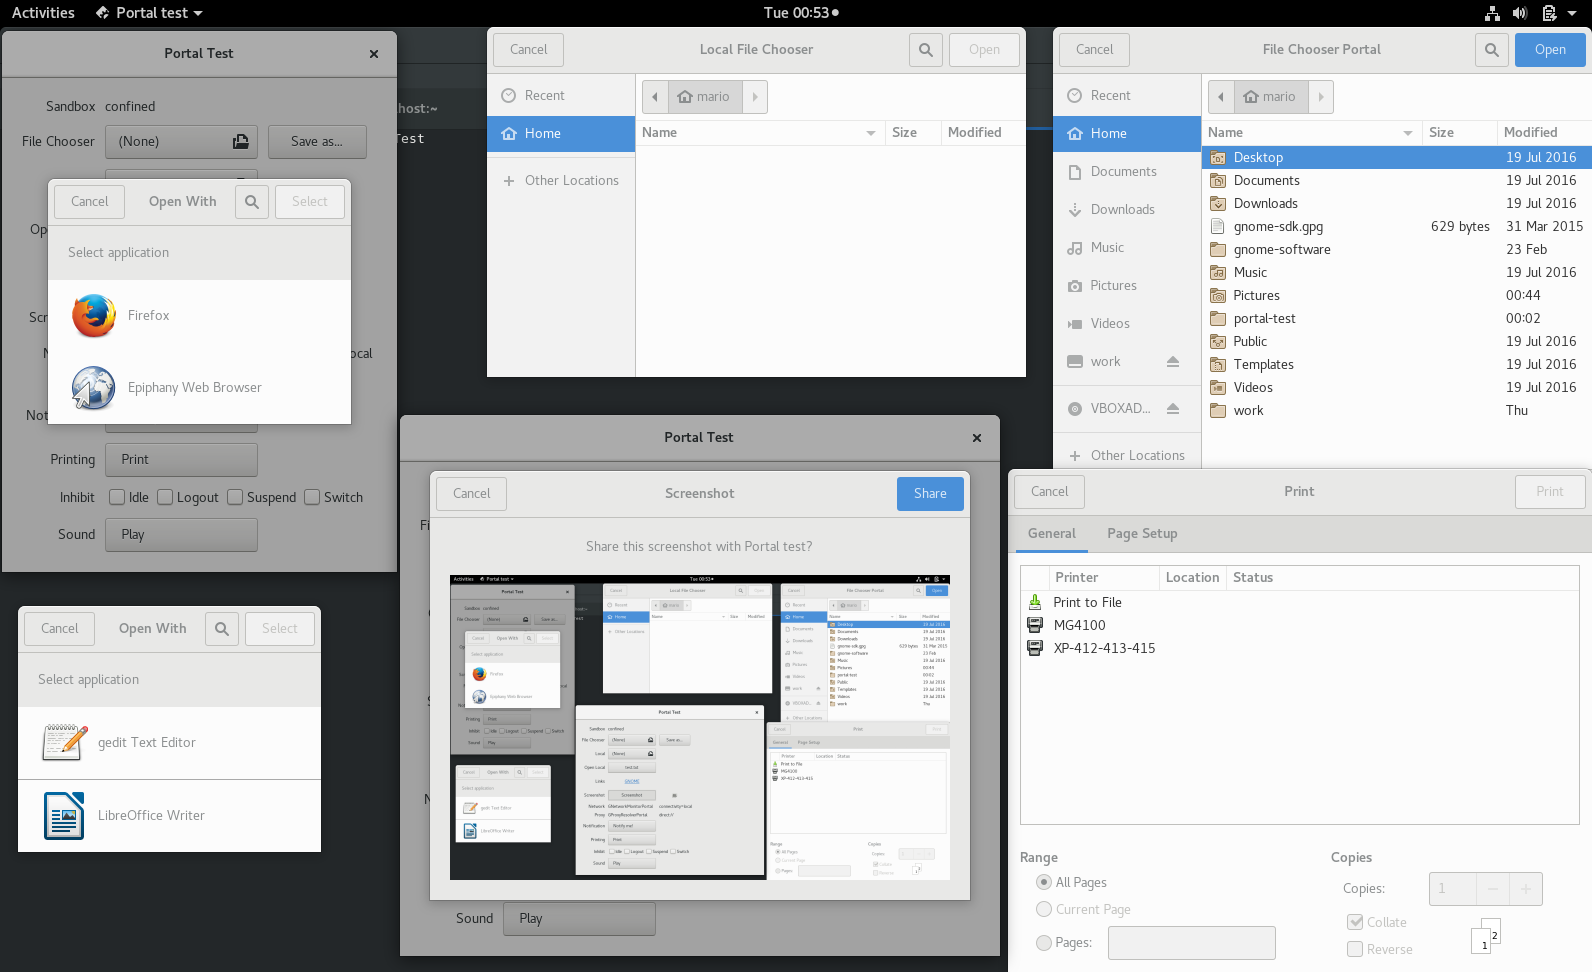
\includegraphics[width=1\textwidth]{images/portals.png}
  \end{center}

\end{frame}

\subsection{Building a flatpak apps}
\begin{frame}[fragile]
  \frametitle{\insertsubsection}

    \begin{tiny}
\begin{verbatim}
{
  "id" : "org.gnome.Todo",
  "branch" : "stable",
  "runtime" : "org.gnome.Platform",
  "runtime-version" : "3.22",
  "sdk" : "org.gnome.Sdk",
  "build-options" : {
    "cflags" : "-O2 -g",
    "cxxflags" : "-O2 -g",
    "env" : {
      "V" : "1"
    }
  },
  "command" : "gnome-todo",
  "modules" : [
    {
      "name" : "gnome-online-accounts",
      "config-opts" : [
        "--disable-telepathy",
        "--disable-documentation",
        "--disable-backend"
      ],
      "sources" : [
        {
          "url" : "https://download.gnome.org/sources/gnome-online-accounts/3.22/gnome-online-accounts-3.22.0.tar.xz",
          "sha256" : "aacce93a71bf5e687a45ae0d00f31ea0625ddd8143235d6d8c64c4ec21bbfa33",
          "type" : "archive"
        }
      ]
    },
    [...] ---> More depedencies here
\end{verbatim}
    \end{tiny}
\end{frame}

\subsection{Building a flatpak apps (II)}
\begin{frame}[fragile]
  \frametitle{\insertsubsection}

    \begin{tiny}
\begin{verbatim}
    [...]
    {
      "name" : "gnome-todo",
      "sources" : [
        {
          "url" : "https://download.gnome.org/sources/gnome-todo/3.22/gnome-todo-3.22.1.tar.xz",
          "sha256" : "cb80f64f5edeeac7b221146d2203bd1bebc49d275b7a41e7a5418f409d9c74af",
          "type" : "archive"
        }
      ]
    }
  ],
  "cleanup" : [
    "/include", "/lib/pkgconfig", "/share/pkgconfig", "/share/aclocal", "/man",
    "/share/man", "/share/gtk-doc", "/share/vala", "*.la", "*.a"
  ],
  "finish-args" : [
    "--share=ipc",
    "--socket=x11",
    "--socket=wayland",
    "--share=network",
    "--talk-name=org.gnome.OnlineAccounts",
    "--talk-name=org.gnome.evolution.dataserver.AddressBook9",
    "--talk-name=org.gnome.evolution.dataserver.Calendar7",
    "--talk-name=org.gnome.evolution.dataserver.Sources5",
    "--talk-name=org.gnome.evolution.dataserver.Subprocess.Backend.*",
    "--filesystem=xdg-run/dconf",
    "--filesystem=~/.config/dconf:ro",
    "--talk-name=ca.desrt.dconf",
    "--env=DCONF_USER_CONFIG_DIR=.config/dconf"
  ]
}
\end{verbatim}
    \end{tiny}
\end{frame}

\subsection{Application distribution}
\begin{frame}
  \frametitle{\insertsubsection}

    \begin{itemize}
    \item Publish your local repository: \texttt{build-export}
      \begin{itemize}
      \item Export your app to an OSTree (archive-z2) repository\vspacing
      \item You could publish this repository now over HTTP\vspacing
      \end{itemize}
    \item Sign everything: \texttt{build-sign}, \texttt{build-update-repo}
      \begin{itemize}
      \item Important to GPG-sign the commits and the summary file\vspacing
      \item Allows using unencrypted HTTP (faster downloads)\vspacing
      \item Recommended to create a dedicated GPG key\vspacing
      \end{itemize}
    \item Push to a production public repository: e.g. \texttt{rsync}
      \begin{itemize}
      \item Simple requirements: static files served over HTTP!\vspacing
      \item Push it to your public server once you're happy\vspacing
      \item Order your commands wisely (avoid race conditions)
      \end{itemize}
    \end{itemize}
\end{frame}

\subsection{Application distribution (II)}
\begin{frame}
  \frametitle{\insertsubsection}

  \begin{itemize}
  \item Configure your public repository appropriately:
    \begin{itemize}
    \item \texttt{build-update-repo --title=<title>}\vspacing
    \item \texttt{build-update-repo --default-branch=<branch>}\vspacing
    \end{itemize}
  \item Provide efficient updates:
    \begin{itemize}
    \item Enable HTTP keep-alive in the server (lots of files)\vspacing
    \item Use OSTree's static-deltas feature (good for big files)\vspacing
    \item Run \texttt{build-update-repo} everytime an app changes\vspacing
    \end{itemize}
  \item Generate application metadata for software centers:
    \begin{itemize}
    \item Generate AppStream data for each application in your repo: \texttt{build-update-repo} will put it an \texttt{appstream} branch\vspacing
    \item Make sure your apps must export an AppData XML file!
    \end{itemize}
  \end{itemize}
\end{frame}

\subsection{Flatpak filetypes: .flatpakrepo and .flatpakref}
\begin{frame}[fragile]
  \frametitle{\insertsubsection}

  \textbf{Configuring flatpak ``repositories''}: \texttt{gnome.flatpakrepo}
  \begin{tiny}
\begin{verbatim}
[Flatpak Repo]
Title=Gnome Stable Runtimes
Url=http://sdk.gnome.org/repo/
Homepage=https://www.gnome.org/get-involved/
Comment=The standard Gnome runtime used by most gnome apps
Description=GNOME runtimes are released with each major release and contain the main GNOME
platform libraries. At the moment they only receive minor bug fixing and security updates,
but should be considered ABI stable and frozen.
Icon=https://www.gnome.org/wp-content/themes/gnome-grass/images/gnome-logo.png
GPGKey=mQENBFUU[...]15w8jmY=
\end{verbatim}
  \end{tiny}

  \textbf{Installing an application}: \texttt{gnome-recipes.flatpakref}
  \begin{tiny}
\begin{verbatim}
[Flatpak Ref]
Title=GNOME Recipes
Name=org.gnome.Recipes
Branch=master
Url=https://matthiasclasen.github.io/recipes-releases/repo
IsRuntime=False
GPGKey=mQENBFis[...]Kpp5G2YW
RuntimeRepo=https://sdk.gnome.org/gnome.flatpakrepo
Comment=GNOME loves to cook
\end{verbatim}
  \end{tiny}

\end{frame}

\subsection{Installing a flatpak application in one click}
\begin{frame}[fragile]
  \frametitle{\insertsubsection}

  GNOME Software, flatpak and \texttt{.flatpakref} files in action:
  \begin{center}
    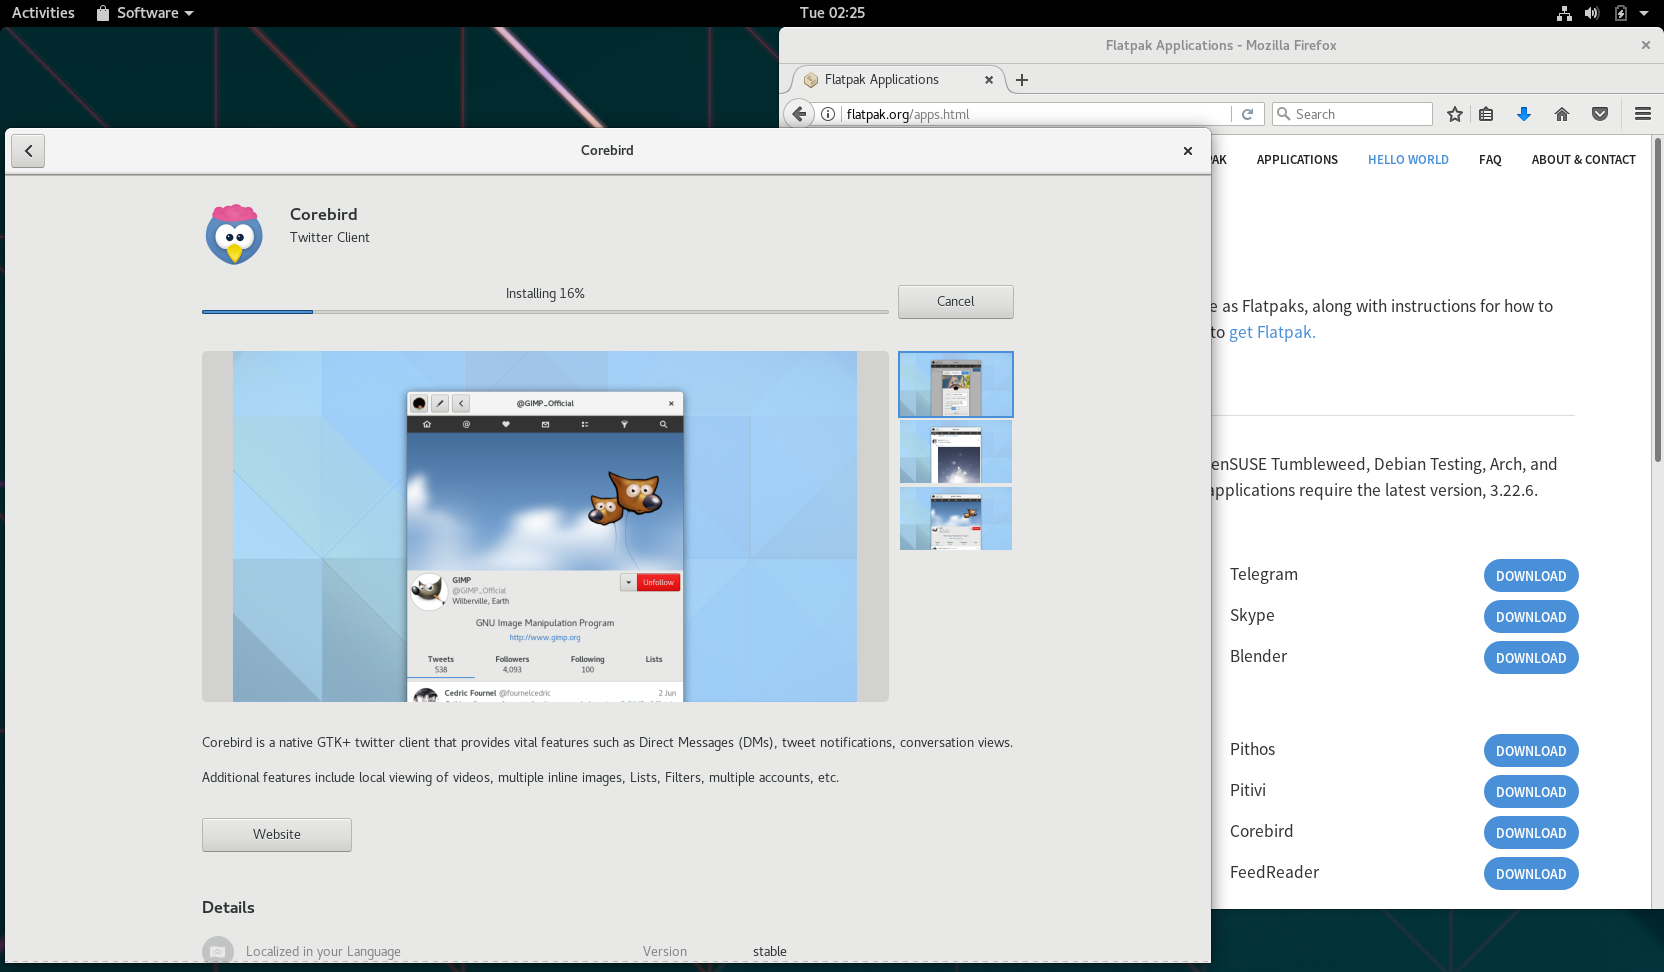
\includegraphics[width=1\textwidth]{images/corebird.png}
  \end{center}

\end{frame}
